\documentclass{article}
\usepackage[T1]{fontenc}
\usepackage{lmodern}
\usepackage{amsmath,amssymb}
\usepackage{tikz}
\usepackage[margin=1in]{geometry}

\begin{document}

%========= Preamble (this is prepended to each question by the importer) =========
\begin{center}
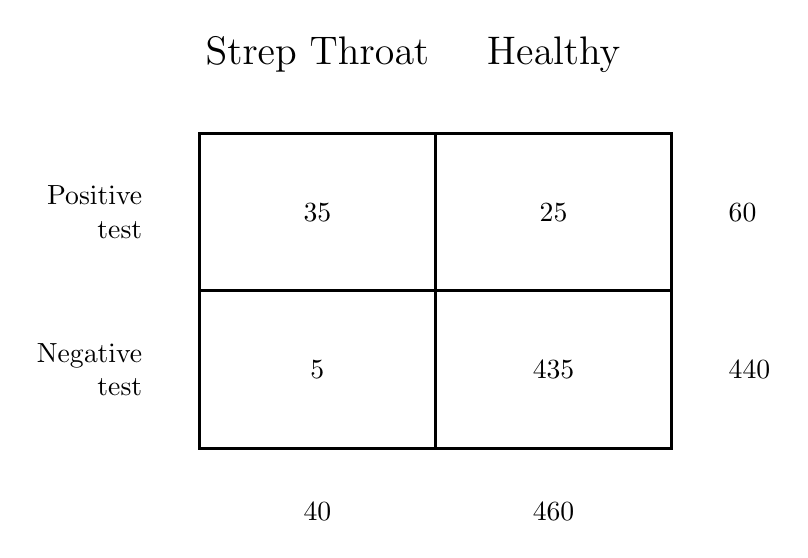
\begin{tikzpicture}[x=1cm,y=1cm]
  % Column titles
  \node[font=\Large] at (1.5,5.0) {Strep Throat};
  \node[font=\Large] at (4.5,5.0) {Healthy};

  % Outer 2x2 box and dividers
  \draw[line width=1pt] (0,0) rectangle (6,4);
  \draw[line width=1pt] (3,0) -- (3,4);
  \draw[line width=1pt] (0,2) -- (6,2);

  % Cell counts
  \node at (1.5,3) {35};
  \node at (4.5,3) {25};
  \node at (1.5,1) {5};
  \node at (4.5,1) {435};

  % Row labels (left of box)
  \node[anchor=east,align=right] at (-0.6,3) {Positive\\test};
  \node[anchor=east,align=right] at (-0.6,1) {Negative\\test};

  % Row totals (to the right of box)
  \node[anchor=west] at (6.6,3) {60};
  \node[anchor=west] at (6.6,1) {440};

  % Column totals (below box)
  \node at (1.5,-0.8) {40};
  \node at (4.5,-0.8) {460};
\end{tikzpicture}
\end{center}

\bigskip
%===============================================================================

\begin{enumerate}[label=\textbf{S\arabic*.}]

% --- S1 ------------------------------------------------------------------------
\item \textbf{Predictive value.} What is the probability that a person has strep
throat \emph{and} tests positive? \answer{B}

\textit{Use the same table above.}

\begin{enumerate}
  \item $\dfrac{35}{500}$
  \item $\dfrac{35}{60}$
  \item $\dfrac{35}{40}$
  \item $\dfrac{35}{35+25+5}$
  \item $\dfrac{35+25+5}{500}$
\end{enumerate}

% --- S2 ------------------------------------------------------------------------
\item \textbf{False-positive rate.} What is the probability of testing positive
\emph{given} that the person does \emph{not} have strep throat? \answer{A}

\textit{Use the same table above.}

\begin{enumerate}
  \item $\dfrac{25}{460}$
  \item $\dfrac{25}{60}$
  \item $\dfrac{35}{40}$
  \item $\dfrac{25}{500}$
  \item $\dfrac{35+25+5}{500}$
\end{enumerate}

% --- S3 ------------------------------------------------------------------------
\item \textbf{Sensitivity.} What is the probability of testing positive
\emph{given} that the person \emph{has} strep throat? \answer{D}

\textit{Use the same table above.}

\begin{enumerate}
  \item $\dfrac{35+25+5}{500}$
  \item $\dfrac{35}{35+25+5}$
  \item $\dfrac{35}{500}$
  \item $\dfrac{35}{40}$    % correct
  \item $\dfrac{35}{60}$
\end{enumerate}

% --- S4 ------------------------------------------------------------------------
\item \textbf{Specificity.} What is the probability of testing negative
\emph{given} that the person does \emph{not} have strep throat? \answer{E}

\textit{Use the same table above.}

\begin{enumerate}
  \item $\dfrac{5}{40}$
  \item $\dfrac{35}{60}$
  \item $\dfrac{35+5+435}{500}$
  \item $\dfrac{435}{500}$
  \item $\dfrac{435}{460}$   % correct
\end{enumerate}

\end{enumerate}

\end{document}








    









